\chapter{卷积神经网络各因素对图像分类的探究}

\section{数据集介绍}

传统的浮游生物调查主要是通过在一块区域内的水采样实现的,但是这种传统方法很难满足目前实际研究的需求,现在的浮游生物研究要求长时间持续性的观察和大规模快速实时的分析,因此目前越来越多的原位浮游生物图像采集系统正在处于开发与使用阶段,例如VPR(Video Plankton Record)\cite{davis2005three}以及SPC(Scripps Plankton Camera)\cite{benfield2007rapid}等设备。科学家们正在不断使用基于图像技术的设备来研究浮游生物的生物特性,通过这些系统或设备,可以很好地研究浮游生物的生态系统。因此,相关机构公开了越来越多的浮游生物图像相关的数据集。下面将介绍三个公开在网络上,使用较为频繁的的浮游生物灰度图像数据集:

\begin{enumerate}
\item ZooScan数据集\footnote{http://www.zooscan.obs-vlfr.fr}

在扫描仪器技术上的快速发展,使短时间内对大量的浮游生物个体进行高质量数字图像化的采集具有可行性和应用性。ZooScan是浮游动物图像扫描分析系统,适用于采集体型微小的浮游生物图像,并且能够快速分析获取图像中浮游生物在形态特征各方面的信息。在这个ZooScan采集到的数据集中,总共有13类浮游动物图像,被分为两个部分:训练集和测试集;其中,训练集图像为9460张图像,测试集为1300张图像。该数据集类别不多,且不同类别的图像数量分布较为平均,图像总数量适中。

\item Kaggle数据集\footnote{https://www.kaggle.com/c/datasciencebowl}

由于浮游生物对地球环境和生态系统的重要性得到越来越多人的关注,但是人工对浮游生物图像的识别与分析的可行性很差,而自动化图像识别分析系统在海洋环境与生态系统的监测中有更广的应用前景。因此,Kaggle组织了国家科学数据杯赛(National Data Science Bowl),要求参赛者对浮游生物图像采取有效的算法实现自动化的图像识别处理,实现浮游生物图像的自动识别与分析。俄勒冈州立大学(Oregon State University)的哈特菲尔德海洋科学中心(Hatfield Marine Science Center)提供了大量的浮游生物图像,有13个种类总共30,000张图像。但是在该数据集中,存在部分浮游生物类别中只有1-2张图像,而有的浮游生物类别图像可达到几千张,是一个非常不平衡的数据集。在这个数据集的基础上,所训练的网络以及分类准确率都不够合理。

\item WHOI-Plankton数据集\footnote{http://darchive.mblwhoilibrary.org/handle/1912/7341 }

伍兹霍尔海洋研究所(Woods Hole Oceanographic Institution)使用了IFCB(The Imaging Flow Cytobot)系统来采集浮游生物图像\cite{orenstein2015whoi}。该系统是一个原位实时系统,从2006年开始就持续性地对浮游生物进行成像处理。到目前为止,该系统已经生成了超过7亿张样本图像。伍兹霍尔海洋研究所发布了一个巨大规模的、基于视觉识别的浮游生物数据集:WHOI-Plankton。该数据集的主要功能就是用于浮游生物分类的相关研究,其包含了70类超过340万张浮游生物图像。这些图像是由IFCB在近8年不断收集到的浮游生物图像数据所组成的。实际上,官方所提供的数据集中,是包含了103类超过300万张浮游生物图像。虽然该数据集在种类丰富度和图像数量上都非常充足,然而这103类浮游生物的数据集中,浮游生物图像的分布是非常不平衡的,其中有一类超过了200百万张图像,有部分浮游生物类别有10万张图像,然而也有的类别图像甚至低于500张。因此通过这种不平衡的数据集训练得到的网络模型,其分类准确率同样是不够合理的。

\end{enumerate}

根据以上三个数据集的规模和特点,以及深度学习实现的要求,在这里本论文选择ZooScan数据集和WHOI-Plankton数据集进行实验。由于ZooScan数据集数量和图像较少,可用来验证卷积神经网络在浮游生物图像分类上的可行性,以及探究影响卷积神经网络在浮游生物图像分类准确率的各个因素;WHOI-Plankton数据集中具有较多的浮游生物图像,以及较多类别的浮游生物,可以用来验证本论文所提出的基于多特征卷积神经网络模型。

%%%%%%%%%%%%%%%%%%%%%%%%%%%%%%%%%%%%%%%%%%%%%%%%%%%%%%%%%%%%%%%%%%%%%%%%%%%%%%%%%%%%%%%%%%%%%
\section{探究网络参数对分类结果的影响}

首先,为了验证深度学习学浮游生物图像分类问题的可行性,考虑到ZooScan数据集的浮游生物种类和数量比较合适,因此将当前流行的卷积神经网络模型应用在ZooScan浮游生物数据集上,并且通过对网络中几个重要的参数进行修改设置,判断卷积神经网络在浮游生物图像数据集上的可行性,以及探讨在卷积神经网络的哪些因素在浮游生物图像数据上起着关键作用。本论文主要从以下四个方面进行实验:数据集图像数量、网络层数,卷积核的尺寸和数量,不同的修正线性单元作用。而对于结果而言,准确率、训练损失值、验证损失值、网络复杂度等都是衡量网络整体性能的重要指标。

在ImageNet数据集上取得了显著效果的卷积网络:AlexNet、CaffeNet、VGGNet和GoogLeNet都被应用在浮游生物数据集上,作为最基础的衡量指标。表一表示了这些网络模型在ZooScan数据集上的分类结果。造成这种结果可能的原因是尽管这些模型在自然场景分类任务下具有非常良好的能力,但是由于数据集本身在质量与数量上的限制,可能造成网络的学习和泛化能力降低,不能取得很好的效果。因此需要分析卷积神经网络的各个因素,对其进行改进提高准确率。这里的实验方法主要是采用自底向上的方法,通过对网络本身性质的探索,在实验的基础上研究出网络关键因素,根据这些因素提出适用于浮游生物数据集分类的卷积神经网络。本实验采用了AlexNet作为基础网络,因为AlexNet是第一个在ImageNet图像大规模视觉识别竞赛中取得优胜的深度学习网络模型,同时也是目前许多网络模型的雏形,可以很好地对其进行改造和设计。

\begin{table}[H]
%\small
\centering
\caption{在ZooScan数据集上,不同卷积神经模型所取得的结果}
\label{comparison}
\vspace{0.2em}
\begin{tabular}{|c|c|c|c|c|c|c|}
\hline 模型 & 准确率 & 训练损失值 & 验证损失值 & 结构 & 训练时间\\ 
\hline AlexNet  & 82.1\% & 0.4273 & 0.5385 & 5 Conv + 3 FC &  8 min\\
\hline CaffeNet & 81.6\% & 0.3422 & 0.5496 & 5 Conv + 3 FC &  8 min\\
\hline VGGNet  & 81.9\% & 0.3921 & 0.5175 & 13 Conv + 3 FC &  14 min\\
\hline GoogleNet & 82.1\% & 0.4618 & 0.5356 & -  & 15 min\\
\hline  
\end{tabular}
\end{table}


\subsection{数据增强}

数据量是深度学习最关键的因素之一,在大量数据的基础上,深度学习可以探索出数据内部所隐藏的最本质的规律,以及表达出数据中最具代表性的模式。然而,因为数据量的缺乏,就算学习能力强的神经网络,也无法探索与表示具有代表性的特征与模式,也就不能取得很好的结果。

由于ZooScan数据集中包含13类浮游生物总共9460张浮游生物图像,虽然对于普通机器学习的方法,这规模的数据集已经有了足够的图像,但是对于深度学习而言,所需要的数据量却仍然是不够的,最后造成的结果可能就是较低的分类准确率以及过拟合现象的发生。因此,必须采取有效的方法提升数据规模,同时这也是最有效的方法来解决训练过程中的过拟合问题,从本质上对深度学习的结果进行提升。

对于浮游生物图像而言,旋转不变性和平移不变性是非常重要的特性,因此这里主要采用了旋转和平移的方法来增加数据集的规模,并且再增加其它几种数据增强方法,使数据更加多样性:

\begin{enumerate}
\item 旋转:随机将图像旋转90度、180度、270度中的任一角度;
\item 平移:随机将图形向水平方向或垂直方向平移40个像素;
\item 缩放:随机将图像中的浮游生物放大或缩小1.2倍;
\item 镜像:随机将图像根据水平方向或者垂直方向进行翻转映射;
\item 斜切:随机将图像由正20度或者负20度的斜切变换;
\end{enumerate}

\begin{figure}[H]
\centering
\begin{minipage}[]{0.3\linewidth} 
      \centering 
      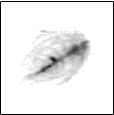
\includegraphics[height=2.5cm]{origin}
        \centerline{(a) 原始图像}\medskip
\end{minipage}
  \begin{minipage}[]{0.3\linewidth}
    \centering
    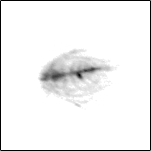
\includegraphics[height=2.5cm]{rotation.png}
      \centerline{(b) 旋转}\medskip
  \end{minipage}
  \begin{minipage}[]{0.3\linewidth}
    \centering
    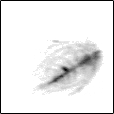
\includegraphics[height=2.5cm]{translation}
      \centerline{(c) 平移}\medskip
  \end{minipage}
\begin{minipage}[]{0.3\linewidth} 
      \centering 
      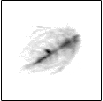
\includegraphics[height=2cm]{resize}
        \centerline{(d) 缩放}\medskip
\end{minipage}
  \begin{minipage}[]{0.3\linewidth}
    \centering
    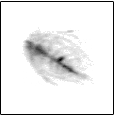
\includegraphics[height=2.5cm]{mirror}
      \centerline{(e) 镜像}\medskip
  \end{minipage}
  \begin{minipage}[]{0.3\linewidth}
    \centering
    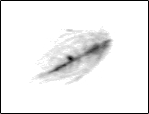
\includegraphics[height=2.2cm]{shearing}
      \centerline{(f) 斜切}\medskip
  \end{minipage}
  \caption{原始图像,以及使用不同数据增强方式得到的结果}
\label{fig:augmentation}
\end{figure}

表~\ref{tab:da}表示不同网络在经过数据增强的数据集上训练后,所得到的结果。从该表中可以看出,各个网络的分类准确率都有大幅度提升。尽管数据增强可以大量地增加图像数量,增加数据集的规模,在结果上,提升了网络的分类准确率;相应地也增加了网络的训练时间。然而在足够强大的硬件条件支持下,所增强的训练时间是能够省略的。

\begin{table}[H]
%\small
\centering
\caption{数据增强后,卷积神经网络在ZooScan数据集上的结果}
\label{tab:da}
\vspace{0.2em}
\begin{tabular}{|c|c|c|c|c|c|c|}
\hline 模型 & 准确率 & 训练损失值 & 验证损失值 & 结构 & 训练时间\\ 
\hline AlexNet  & 91.3\% & 0.0122 & 0.2263 & 5 Conv + 3 FC  & 28 min \\
\hline CaffeNet & 91.0\% & 0.0775 & 0.2435 & 5 Conv + 3 FC  & 28 min \\
\hline VGGNet  & 92.2\% & 0.0144 & 0.2011 & 13 Conv + 3 FC  & 54 min \\
\hline GoogleNet & 91.9\% & 0.0041 & 0.2454 & - &  57 min \\
\hline  
\end{tabular}
\end{table}



\subsection{网络深度}
近期相应的研究表明,网络的深度是主导其在数据集上性能的主要因素。网络深度也表示了深度学习的学习能力,越深的网络其学习能力越强。近些年在ImageNet数据集上取得优胜的深度学习网络模型都有非常深层次的网络结构。这也表示了网络的深度,即网络层数,是影响网络结果的最关键因素之一。因此,将网络从8层到16层的逐层拓展,可以得到不同的结果,通过观察与比较这些结果来推导出最后的结论。根据VGGNet网络的实验结论,将一些小卷积核的卷积层堆积起来,而不是使用一个大卷积核的卷积层,可以很好地增加网络的深度,而且还能降低网络参数、容量的消耗以及庞大的计算量。在这里,对于改进网络深度同样使用了卷积层堆积的方法。

\begin{table}[H]
%\small
\centering
\caption{在ZooScan数据集上,关于网络深度实验的五种网络结构形式}
\label{tab:config}
%\vspace{0.2em}
\begin{tabular}{|c|c|c|c|c|c|}
\hline 8层(AlexNet) & 9层 & 11层 & 13层 & 16层 \\ 
\hline \multicolumn{5}{|c|}{input (227 $\times$ 227 image crop)} \\
\hline \multirow{2}{*}{conv11-96} & \multirow{2}{*}{conv11-96} & \multirow{2}{*}{conv11-96} & \multirow{2}{*}{conv11-96} & conv7-96 \\
	& & & & conv7-96 \\
\hline \multicolumn{5}{|c|}{3$\times$3 maxpool} \\
\hline \multirow{2}{*}{conv5-256} & \multirow{2}{*}{conv5-256} & \multirow{2}{*}{conv5-256} & \multirow{2}{*}{conv5-256} & conv3-256 \\
	& & & & conv3-256 \\
\hline \multicolumn{5}{|c|}{3$\times$3 maxpool} \\
\hline conv3-384 &  conv3-384 & conv3-256 & conv3-256 & conv3-256 \\

	conv3-384 & conv3-384 & conv3-256 & conv3-256 & conv3-256  \\

	conv3-256 & & conv3-256 & & conv1-256 \\
	\cline{1-5} \multicolumn{5}{|c|}{3$\times$3 maxpool} \\
	\cline{1-5} &  conv3-384 & conv3-384 & conv3-384 & conv3-384 \\
	& conv3-384 & conv3-384 & conv3-384 & conv3-384  \\
	&  &  conv3-384 & conv1-384 & conv1-384 \\
	\cline{2-5} &  \multicolumn{4}{c|}{3$\times$3 maxpool} \\
	\cline{1-5} & & & conv3-384 & conv3-384 \\
	 & & & conv3-384 & conv3-384 \\
	& & & conv1-384 & conv1-384 \\
	\cline{4-5} & & & \multicolumn{2}{|c|}{3$\times$3 maxpool}\\

\hline \multicolumn{5}{|c|}{FC-4096}\\
\hline \multicolumn{5}{|c|}{FC-4096}\\
\hline \multicolumn{5}{|c|}{FC-13}\\
\hline \multicolumn{5}{|c|}{softmax layer} \\
\hline  
\end{tabular}
\end{table}

\begin{table}[H]
%\small
\centering
\caption{不同深度的网络在ZooScan数据上的结果}
\label{tab:dep}
\begin{tabular}{|c|c|c|c|c|c|c|c|}
\hline 模型 & 准确率 & 训练损失值 & 验证损失值 & 训练时间\\ 
\hline 8层 & 91.3\% & 0.0122 & 0.2263 & 28 min \\
\hline 9层 & 92.1\% & 0.0201 & 0.2255 & 29 min \\
\hline 11层 & 92.8\% & 0.0401 & 0.2722 & 34 min \\
\hline 13层 & 92.5\% & 0.0415 & 0.2612 & 44 min  \\
\hline 16层 & 92.3\% & 0.0455 & 0.2627 & 53 min  \\
\hline
\end{tabular}
\end{table}

表~\ref{tab:dep}表示在数据增强的前提下,不同深度的网络所得到的准确率结果。表~\ref{tab:config}表示不同网络深度下的网络结构设置,因为采用了卷积层堆积的方法,所以深度不是线性增长的。从表~\ref{tab:dep}中可以看出,在很高的分类准确率的前提下,网络深度的改进只能小幅度地提升网络性能。但是,随着网络的持续增加,在训练过程中将会消耗更多的时间,最后准确率反而还下降了。导致这种情况的发生,可能是由于梯度的消失或爆炸。


\subsection{网络宽度}
网络的宽度,即卷积层中卷积的大小和数量,是除了网络深度外,另一个影响网络学习能力的因素。在实验中,我们试过了许多不同尺寸的卷积核:13x13,11x11,7x7,甚至是三个5x5的堆积,来寻找合适大小的卷积核。而不同的卷积核数量256,384和512,也是我们考虑的另外一个方面。

表~\ref{tab:width}表示了不同卷积核设置下的图像分类结果。由于之前的结果表示11层卷积神经网络在浮游生物数据上能取得较好结果,因此对于网络宽度的修改,是基于11层网络为基础的。表~\ref{tab:width}第二列表示基础网络,随后各列表示不同宽度的网络配置,分别以A、B、C和D命名,各个网络的层数相同,只是卷积核的大小和数量不同。正常来说,11x11和7x7大小的卷积核在分类任务上可以取得很好的结果。但是在浮游生物图像分类上,将第一层卷积核设置为13x13,第二层卷积核设置为7x7,反而能取得很好的结果,相应也会带来计算量增大以及网络复杂度的增加。对此结果的推断是:由于图像只有浮游生物,因此大尺寸的卷积核能获取更多关于浮游生物有用的信息。相似地,更多数量的卷积核从更多维度来获取特征,因此384和512的卷积数量设置能够取得很好的结果。


\begin{table}[H]
%\small
\centering
\caption{不同大小和不同数量的卷积核的网络在ZooScan数据集上的结果}
\label{tab:width}
\begin{tabular}{|c|c|c|c|c|c|c|c|c|}
\hline  & 11层 & A & B & C & D \\ 
\hline \multirow{10}{*}{网络结构}& conv11-96 & conv13-96 & conv13-96 & conv13-96 & conv13-96 \\
	& & & & &  \\
	\cline{2-6} & conv5-256 & conv5-256 & conv7-256 & conv7-256 & conv7-256 \\
	& & & & & \\
	\cline{2-6} & conv3-256 & conv3-256 & conv3-256 & conv3-384 & conv3-512 \\
        & conv3-256 & conv3-256 & conv3-256 & conv3-384 & conv3-512 \\
        & conv3-256 & conv3-256 & conv3-256 & conv3-384 & conv3-512 \\
	& & & & & \\
	\cline{2-6} & conv3-384 & conv3-384 & conv3-384 & conv3-512 & conv3-512 \\
	& conv3-384 & conv3-384 & conv3-384 & conv3-512 & conv3-512 \\
	& conv3-384 & conv3-384 & conv3-384 & conv3-512 & conv3-512 \\
	& & & & & \\
\hline 准确率 & 92.8\% & 92.9\% & 93.1\% & 93.6\% & 93.6\% \\
\hline 训练时间 & 34 min & 35 min & 36 min & 39 min & 43 min \\
\hline 
\end{tabular}
\end{table}

\subsection{线性修正单元}
线性修正单元(Rectified Linear Units, ReLU)作为深度学习网络中的激活函数,起着非常重要的作用,保证了网络的正常训练。ReLU在训练过程中加速了收敛,代替了传统的sigmoid函数作用于当前的深度网络结构中。另外一些研究学者更关注修正单元的功能,提出了PReLU(Parametric ReLU)取代普通的ReLU模块,其可以逐步学习改进修正单元的参数。相比较于使用ReLU的卷积网络,使用PReLU的卷积网络在可忽略的额外计算量代价下,提升了最后的准确率。最终结果表示在表~\ref{tab:re}中,该结果是以表~\ref{tab:width}中11层网络结构的C配置为基础展开的。尽管PReLU在训练时间和准确率上只有轻微的影响,但是其仍然能够起到一定作用。

\begin{table}[H]
%\small
\centering
\caption{包含ReLU和PReLU的网络结构C在ZooScan数据集上的准确率}
\label{tab:re}
\begin{tabular}{|c|c|c|c|}
\hline 结构 & 准确率 & 训练时间\\
\hline C (ReLU) & 93.6\% & 39 min \\
\hline C (PReLU) & 93.7\% & 38 min \\
\hline 
\end{tabular}
\end{table}

通过以上多组实验,以及对实验结果的分析和讨论,可以得出:基于深度学习的卷积神经网络,可作为浮游生物图像分类问题的解决方案。影响浮游生物图像分类准确率的最主要因素是图像的数据增强;通过数据增强,可以提升数据集的多样性,保证网络充分训练;其次,卷积神经网络的深度与宽度同样是非常重要的因素,通过对深度和宽度的控制,虽然训练时间有所增加,但是仍然能提升图像的分类准确率。但是由于经过数据增强的提升,基础网络准确率已经达到很高的水准,因此通过对网络深度和宽度的修改,只能小幅度地提升结果;最后,对卷积神经网络中的激活函数和线性修正单元的改进,只是很小幅度地提升实验结果。因此,从上述实验结果,再次验证数据增强、网络深度和宽度是影响网络性能的最主要因素,对于浮游生物图像分类的结果同样适用。


%\begin{figure}[H] % use float package if you want it here
%  \centering
%  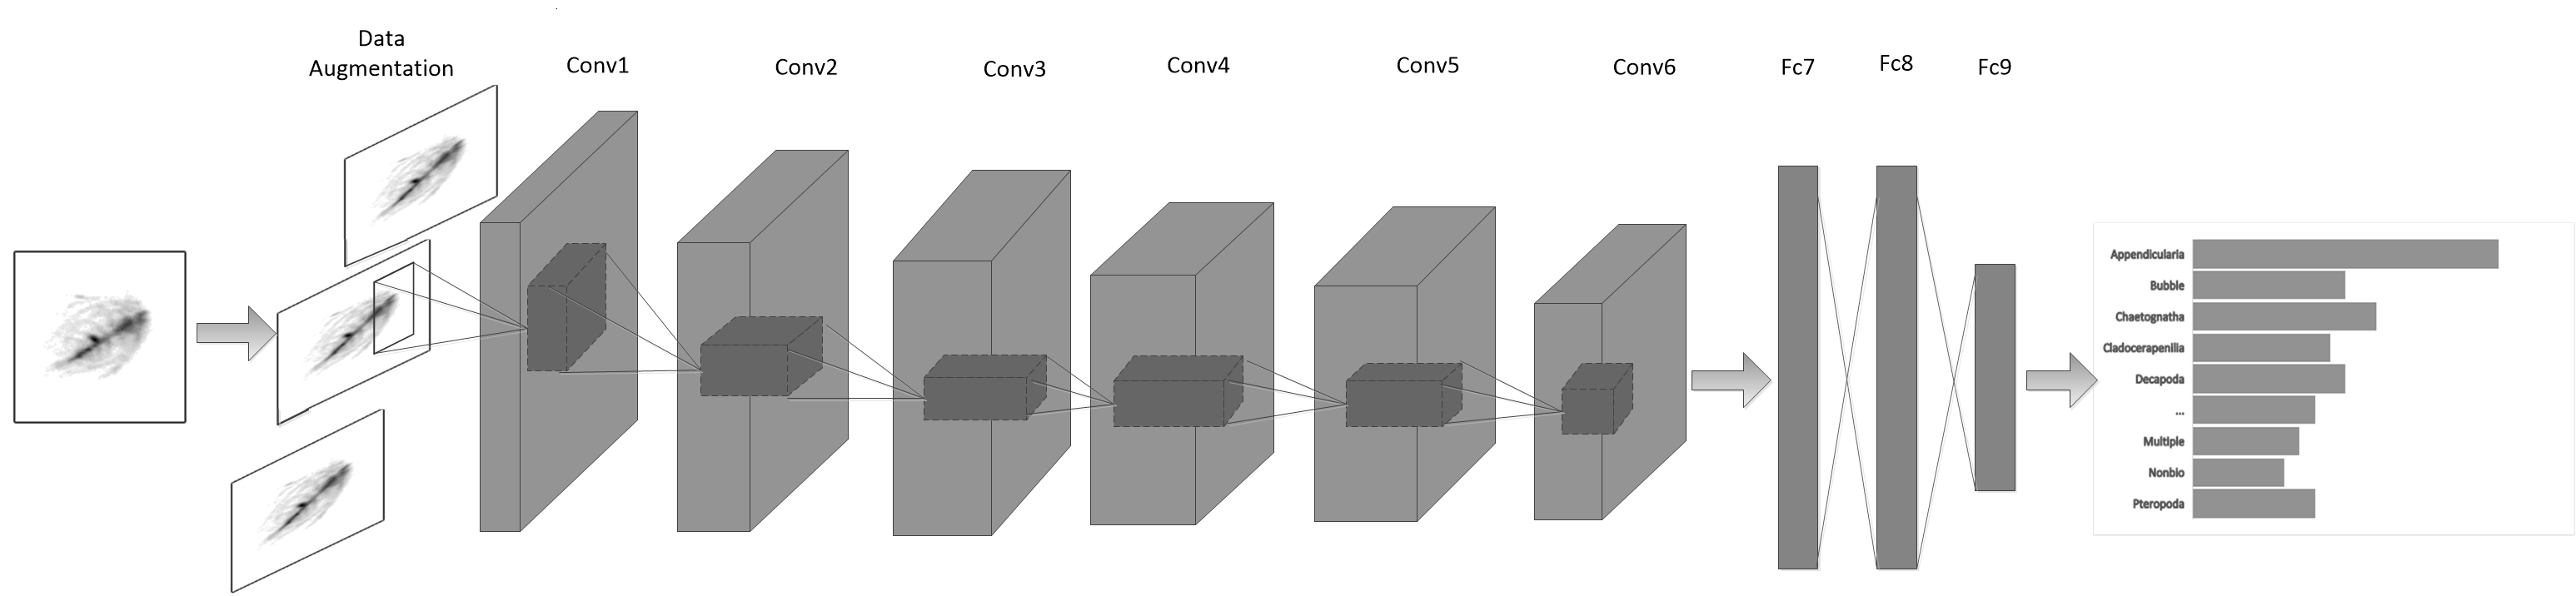
\includegraphics[height=3.8cm]{network}
%  \caption{对上述因素总结,所提出的基于浮游生物图像的单卷积神经网络模型}
%  \label{fig:xfig1}
%\end{figure}

%%%%%%%%%%%%%%%%%%%%%%%%%%%%%%%%%%%%%%%%%%%%%%%%%%%%%%%%%%%%%%%%%%%%%%%%%%%%%%%%%%%%%%%%%%%%%
\section{组合网络模型}

根据以上所得到的实验结果,AlexNet在网络的深度和宽度与其他卷积伸进网络模型相比,具有较大的改进空间和潜力,本章在AlexNet的基础上对应其进行改进和总结。根据之前网络深度和网络宽度的实验结果,对AlexNet进行修改,加上数据增强和改进线性修正单元,可总结得到应用于少量类别的浮游生物图像分类的卷积神经网络模型,称为ZooplanktoNet。由于该模型是基于13类浮游生物图像数据集进行训练的,因此只能应用于少量类别的浮游生物图像分类。图~\ref{fig:stack}表示该模型的具体结构。

\begin{figure}[H] % use float package if you want it here
  \centering
  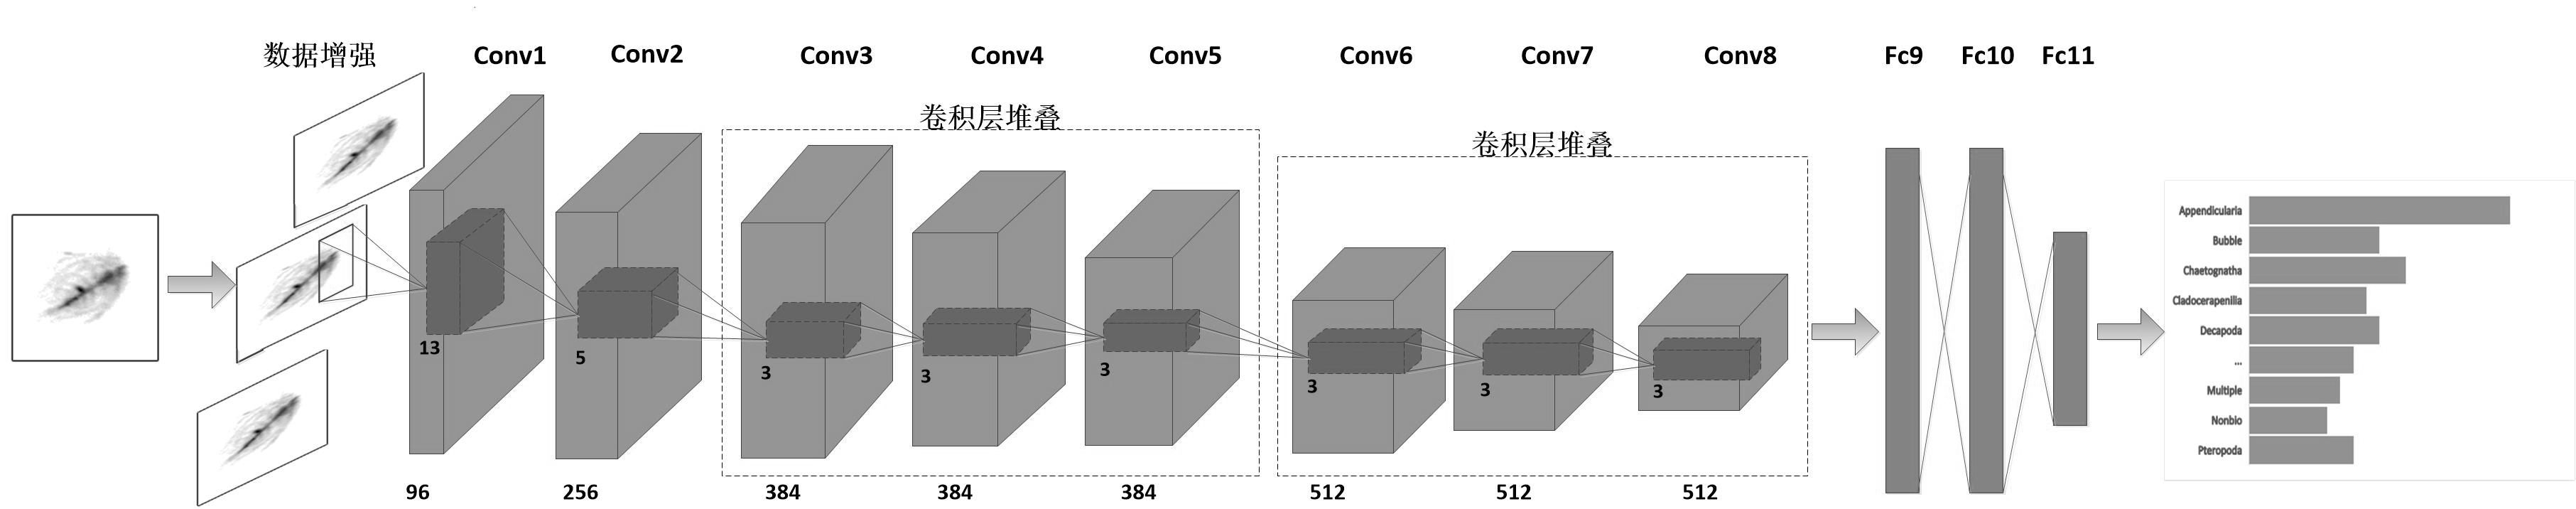
\includegraphics[height=3cm]{stack}
  \caption{应用于少量类别的浮游生物图像分类的卷积神经网络模型ZooplanktoNet}
  \label{fig:stack}
\end{figure}

首先,浮游生物图像数据集使用数据增强方法,扩大训练数据的规模;随后,训练数据经过8层卷积层和3层全连接层组成的卷积神经网络模型(其中,卷积层的卷积核大小和数量,随层数的增加,相应地减少和增大;且相邻的三个卷积层组成卷积层堆叠);最后,末尾的全连接层输出网络预测结果。表~\ref{tab:re}中的第二行实验数据,就是ZooplanktoNet在数据集上的分类结果。

通过以上实验证明,卷积神经网络模型ZooplanktoNet针对13类浮游生物图像,其准确率超过ZooScan扫描仪所能达到的最高准确率,能够有效解决少量类别的浮游生物图像分类问题。

%%%%%%%%%%%%%%%%%%%%%%%%%%%%%%%%%%%%%%%%%%%%%%%%%%%%%%%%%%%%%%%%%%%%%%%%%%%%%%%%%%%%%%%
\section{本章总结}

本章节主要介绍了浮游生物相关的数据集、在浮游生物图像分类中卷积神经网络性能影响因素的探究、以及提出了应用于浮游生物图像分类的卷积神经网络模型。根据所设置的多组实验的结果进行分析,证明数据增强、网络深度和宽度同样是影响卷积神经网络对浮游生物图像分类结果的最主要因素。另外,本章还将对这些结果进行总结,启发性地提出了一个应用于少量类别的浮游生物图像分类的卷积神经网络模型,在保证准确率和训练条件的前提下,能够有效实现图像的分类。












